% !TeX program = xelatex
\documentclass[UTF8,fontset=fandol,10pt,a4paper]{ctexart}
\usepackage[left=22mm,right=22mm,top=23mm,bottom=22mm,headheight=14pt]{geometry}
\usepackage{fontspec}
\setmainfont{TeX Gyre Heros}
\setsansfont{TeX Gyre Heros}
\setmonofont{Latin Modern Mono}
\renewcommand{\familydefault}{\sfdefault}
\usepackage[table]{xcolor}
\usepackage{graphicx,tikz}
\usetikzlibrary{arrows.meta,positioning,fit,backgrounds,calc}
\usepackage{booktabs,tabularx,array,enumitem,float,caption,fancyhdr,hyperref}
\definecolor{blue}{HTML}{2869A9}
\definecolor{ink}{HTML}{293340}
\definecolor{muted}{HTML}{647181}
\definecolor{line}{HTML}{C5D4E2}
\definecolor{pale}{HTML}{F0F5FA}
\definecolor{warm}{HTML}{FFF7E9}
\hypersetup{colorlinks=true,urlcolor=blue,linkcolor=blue,pdftitle={Redflag RHI 与 Vulkan 接入设计},pdfauthor={Redflag}}
\color{ink}
\setlength{\parindent}{0pt}
\setlength{\parskip}{6pt}
\linespread{1.16}
\setlist[itemize]{leftmargin=1.5em,itemsep=2pt,topsep=3pt}
\setlist[enumerate]{leftmargin=1.8em,itemsep=3pt,topsep=3pt}
\renewcommand{\arraystretch}{1.38}
\newcolumntype{Y}{>{\raggedright\arraybackslash}X}
\newcolumntype{L}[1]{>{\raggedright\arraybackslash}p{#1}}
\ctexset{section={format=\Large\bfseries\color{blue},beforeskip=16pt,afterskip=8pt},subsection={format=\large\bfseries\color{blue},beforeskip=11pt,afterskip=5pt}}
\captionsetup{font=small,labelfont=bf,textfont={color=muted},skip=7pt}
\pagestyle{fancy}\fancyhf{}
\fancyhead[L]{\small\color{muted}Redflag · RHI / Vulkan · 设计方案}
\fancyhead[R]{\small\color{muted}2026-11-21}
\fancyfoot[C]{\small\color{muted}\thepage}
\renewcommand{\headrulewidth}{0pt}
\newcommand{\note}[1]{{\small\color{muted}#1\par}}
\newcommand{\code}[1]{{\small\texttt{#1}}}
\newcommand{\ruleline}{\par\vspace{4pt}{\color{line}\hrule}\vspace{8pt}}
\newcommand{\source}[2]{{\small\href{#1}{[#2]}}}
\tikzset{
 module/.style={draw=line,fill=pale,rounded corners=2pt,align=center,inner sep=7pt,text width=3.8cm,minimum height=1.15cm,font=\small},
 smallbox/.style={module,text width=2.55cm,minimum height=.95cm,font=\footnotesize},
 wide/.style={module,text width=9.5cm},
 planned/.style={module,fill=warm,dashed},
 flow/.style={-{Stealth[length=2mm]},draw=muted,line width=.65pt},
 own/.style={flow,dashed},
 label/.style={font=\scriptsize,fill=white,inner sep=2pt,text=muted}}

% 本册的页幅、图注和代码排版。
\geometry{paperwidth=190mm,paperheight=252mm,left=21mm,right=21mm,
  top=22mm,bottom=21mm,headheight=21pt,headsep=4mm,footskip=10mm}
\usepackage{amsmath,listings,type1cm}
\definecolor{Ink}{HTML}{202E33}
\definecolor{Muted}{HTML}{4C6064}
\definecolor{Teal}{HTML}{12665F}
\definecolor{Rust}{HTML}{9E452B}
\definecolor{Rule}{HTML}{B3C6C1}
\definecolor{Soft}{HTML}{EAF3F0}
\definecolor{Paper}{HTML}{FFFFFF}
\setmainfont{TeX Gyre Pagella}
\renewcommand{\familydefault}{\rmdefault}
\linespread{1}
\setcounter{secnumdepth}{0}
\setlength{\emergencystretch}{2em}
\setlength{\parindent}{0pt}
\setlength{\parskip}{5.8pt}
\ctexset{section={format=\raggedright\sffamily\bfseries\fontsize{23}{30}\selectfont\color{Ink},
    beforeskip=0pt,afterskip=9pt},
  subsection={format=\raggedright\sffamily\bfseries\fontsize{13}{18}\selectfont\color{Teal},
    beforeskip=8pt,afterskip=2pt}}
\hypersetup{urlcolor=Teal,linkcolor=Teal,bookmarksnumbered=false,
  pdfsubject={Redflag 渲染接口、后端实现与验证}}
\fancyhf{}
\setlength{\headwidth}{\textwidth}
\fancyhead[L]{\sffamily\fontsize{9.5}{12}\selectfont\bfseries\color{Teal}Redflag\enspace{\mdseries\color{Muted}图形引擎}}
\fancyhead[R]{\sffamily\small\color{Muted}RHI / Vulkan}
\renewcommand{\headrule}{\hbox to\headwidth{\color{Rule}\leaders\hrule height .55pt\hfill}}
\fancyfoot[L]{\small\sffamily\color{Muted}\nouppercase{\leftmark}}
\renewcommand{\sectionmark}[1]{\markboth{#1}{}}
\fancyfoot[R]{\large\sffamily\bfseries\color{Teal}\thepage}
\renewcommand{\code}[1]{{\ttfamily\fontsize{10.4}{14}\selectfont #1}}
\newcommand{\readings}[1]{\par\noindent{\sffamily\fontsize{9.6}{14}\selectfont
  \color{Muted}参考\enspace #1\par}}
\newcommand{\refitem}[2]{\href{#1}{#2}}
\newcommand{\figpanel}[2]{\begin{figure}[H]\centering\input{figures/#1}\caption{#2}\end{figure}}
\DeclareCaptionFont{rhicapt}{\sffamily\fontsize{10}{14}\selectfont\color{Muted}}
\captionsetup{font=rhicapt,labelfont={bf,color=Teal},textfont=rhicapt,
  labelsep=quad,justification=raggedright,singlelinecheck=false,skip=4pt}
\setlength{\intextsep}{7pt plus 1pt minus 1pt}
\lstset{basicstyle=\ttfamily\fontsize{10.7}{15}\selectfont\color{Ink},
  backgroundcolor=\color{Soft},frame=l,rulecolor=\color{Teal},framerule=1.5pt,
  xleftmargin=5mm,xrightmargin=2mm,framexleftmargin=3mm,framesep=2pt,
  aboveskip=6pt,belowskip=6pt,columns=fullflexible,keepspaces=true,showstringspaces=false}
\newcommand{\bodytype}{\normalfont\fontsize{11.4}{17.8}\selectfont\color{Ink}}

\geometry{a4paper,left=23mm,right=23mm,top=22mm,bottom=22mm}
\setlength{\headwidth}{\textwidth}
\fancyhead[R]{\small\sffamily\color{Muted}源码阅读 · 常用接口}
\hypersetup{pdftitle={Redflag 源码阅读：引擎与图形库接口}}
\ctexset{section={afterindent=true},subsection={afterindent=true,beforeskip=10pt,afterskip=4pt}}
\newcommand{\src}[2]{\href{run:../../#1}{\textsf{#2}}}
\lstset{escapeinside={(*@}{@*)}}
\begin{document}
\fontsize{12.7}{20}\selectfont\setlength{\parindent}{2\ccwd}\setlength{\parskip}{8pt}

\section{中庭模型与拾取}
在 Sponza 的场景视图里点一下石柱，右侧属性显示的是整座中庭。再点旁边的拱门，仍然选中同一个物体。中庭是作为一个模型导入的。它的石柱、地板和挂毯分属不同的网格和材质，场景里却只有一个建筑实体。画进屏幕的像素可以有千百种颜色，写给鼠标拾取的都是这个实体的编号。

\begin{figure}[H]\centering
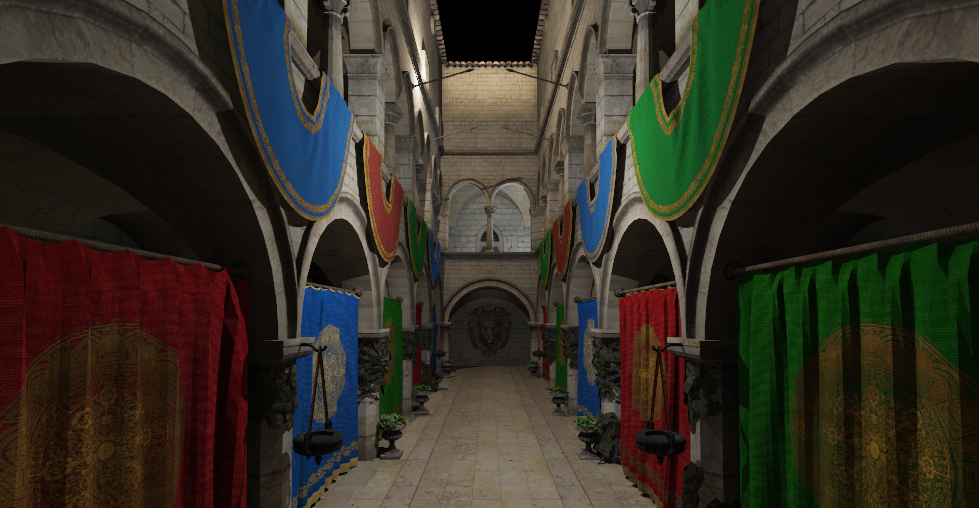
\includegraphics[height=42mm]{../editor-guide/figures/atrium.png}
\caption{编辑器实拍。走廊两侧的拱门、柱面和布帘都来自同一份中庭模型。}
\end{figure}

场景文件用一个资产编号指代中庭的模型。加载时，\code{AssetManager::Load<Model>(id)} 根据编号取回模型。尖括号里的 \code{Model} 是 C++ 模板实参，告诉函数这次需要哪种对象。第一次从文件读取，以后再打开就可以从缓存取得它。网格保存顶点和索引，材质保存底色和贴图。两个实体摆放同一模型时，各自保存位置，共用模型数据。查登记与加载，打开 \src{Redflag/src/Redflag/Assets/AssetManager.h}{AssetManager.h}；要追踪谁交出顶点，打开 \src{Redflag/src/Redflag/Renderer/Mesh.cpp}{Mesh.cpp}。

模型留在内存里，接下来的许多帧都能继续画它。窗口可绘制时，引擎在 \code{Application::Run} 中开始一帧。\code{BeginFrame} 成功后，各层依次进入更新与界面绘制。对应的方法叫 \code{OnUpdate} 和 \code{OnImGuiRender}。编辑器在后一个入口排出面板，得到场景图该画多大，再录制画场景与显示界面的工作。窗口的 \code{OnUpdate} 调用 GLFW 的 \code{glfwPollEvents()} 处理待派送的输入事件，也调用当前图形上下文的 \code{SwapBuffers}。在 Vulkan 实现中还能找到负责提交与呈现的调用。查一帧的顺序，打开 \src{Redflag/src/Redflag/Core/Application.cpp}{Application.cpp}。

到了绘制这一步，\code{SceneRenderer::DrawGeometry} 从同一个建筑实体取出网格和材质，配上各自的变换。画石柱和画挂毯时，它把同一个实体编号交给命令列表。\code{RenderDevice::CreateMesh} 提供可重复使用的几何资源，\code{CommandList::DrawIndexed} 则描述这一次使用哪份网格、贴图、相机与模型矩阵。跟进命令列表里的函数，会看到 OpenGL 与 Vulkan 两种写法。\par
\readings{\src{Redflag/src/Redflag/Renderer/SceneRenderer.cpp}{SceneRenderer.cpp}\quad
\src{Redflag/src/Redflag/Renderer/RHI/CommandList.h}{CommandList.h}\quad
\href{https://www.glfw.org/docs/3.3/quick_guide.html}{GLFW 作者指南}\quad
\href{run:../api/index.html}{离线 API 索引}}

\clearpage
\section{三角形的索引}
暂时把建筑简化成一面正方形的墙。它有四个顶点，编号为 $0,1,2,3$。索引数组按 $0,1,2,\,2,3,0$ 排列，每三个数构成一个三角形。因此本次绘制传入的索引数是 6。顶点 0 和 2 被取了两次，数组里仍只存一份该顶点的位置与贴图坐标。

\begin{figure}[H]\centering
\begin{tikzpicture}[x=1mm,y=1mm,every node/.style={font=\small\sffamily,text=Ink}]
  \draw[rounded corners=1.4mm,draw=Rule] (0,0) rectangle (144,36);
  \filldraw[fill=Teal!14,draw=Teal] (12,5)--(40,5)--(40,31)--cycle;
  \filldraw[fill=Rust!12,draw=Rust] (12,5)--(40,31)--(12,31)--cycle;
  \foreach \x/\y/\t in {8/5/0,44/5/1,44/31/2,8/31/3}{\node at (\x,\y){\t};}
  \node[anchor=west,text=Teal] at (53,24){第一个三角形\qquad 0\quad 1\quad 2};
  \node[anchor=west,text=Rust] at (53,12){第二个三角形\qquad 2\quad 3\quad 0};
\end{tikzpicture}
\caption{两片三角形共用对角线上的顶点 0 和 2。数字是顶点在数组里的序号。}
\end{figure}

在 \code{OpenGLCommandList::DrawIndexed} 里，先选用材质着色器，写入相机与模型矩阵、底色和实体编号。贴图的 \code{Bind(0)} 最终调用 \code{glBindTextureUnit}，即让着色器从编号为 0 的纹理单元读当前这张图。绑定网格后，\code{RenderCommand} 把请求送到 \src{Redflag/src/Platform/OpenGL/OpenGLRendererAPI.cpp}{OpenGLRendererAPI.cpp} 的 \code{DrawIndexed}。
\begin{lstlisting}
// (*@这里传索引个数。墙上两个三角形共用六个索引。@*)
glDrawElements(GL_TRIANGLES, count, GL_UNSIGNED_INT, nullptr);
\end{lstlisting}
驱动读到这条命令时，\code{count} 给出要取的索引个数，\code{GL\_UNSIGNED\_INT} 指每个索引用一个 32 位无符号整数。最后的空指针在绑定了索引缓冲区的前提下表示从第 0 字节开始读。另一个常见函数 \code{glNamedBufferSubData} 直接按缓冲区的 OpenGL 名称写入数据。\code{offset} 与 \code{size} 都按字节计算。哪个着色器会看到这份数据，还取决于绘制时它能从哪里读取。

换到 Vulkan，同样六个索引仍然画出这面墙。在 \src{Redflag/src/Platform/Vulkan/VulkanDraw.cpp}{VulkanDraw.cpp} 的 \code{DrawIndexed} 里能找到同一笔绘制。
\begin{lstlisting}
// (*@录入 cmd；后端提交它后，显卡才会画这面墙。@*)
vkCmdDrawIndexed(cmd, mesh.IndexCount, 1, 0, 0, 0);
\end{lstlisting}
\code{cmd} 保存正在录制的命令；本例索引数为 6、实例数为 1。后三个 0 分别指定从第 0 个索引开始、顶点编号不额外偏移、实例序号从 0 开始。前面的 \code{vkCmdBindVertexBuffers}、\code{vkCmdBindIndexBuffer} 和 \code{vkCmdBindDescriptorSets} 分别指定读哪份顶点、索引和材质贴图。后端用 \code{vkCmdPushConstants} 把本次绘制的矩阵、颜色与实体编号记入命令，稍后 \code{vkQueueSubmit} 才把录好的工作交给队列。
\readings{\src{Redflag/src/Platform/OpenGL/OpenGLCommandList.cpp}{OpenGLCommandList.cpp}\quad
\src{Redflag/src/Platform/Vulkan/VulkanDraw.cpp}{VulkanDraw.cpp}\\
\href{https://github.com/KhronosGroup/OpenGL-Refpages/blob/main/gl4/glDrawElements.xml}{Khronos · glDrawElements}\quad
\href{https://docs.vulkan.org/refpages/latest/refpages/source/vkCmdDrawIndexed.html}{Khronos · vkCmdDrawIndexed}}

\clearpage
\section{实时效果与计算着色器}
在「实时效果」中勾选 GTAO，再看 Sponza 柱脚与地面的交界。合成视图会用一个可见度值压暗周围遮住的间接光。如果这里一直和开关前一样亮，可以从复选框跟到那张可见度图，看改变停在哪一步。

\code{ImGui::Checkbox(label, \&m\_AO)} 的第一个参数是显示文字，第二个参数指向保存开关的布尔变量。函数返回值表示用户本次是否改变了选项，变量本身表示改变之后的开关状态。界面合并多个控件的变化后重置历史，否则上一种设置算出的颜色还会混进来。要找这些开关，打开 \src{RedflagForge/src/LightingPreview.cpp}{LightingPreview.cpp}。

\begin{figure}[H]\centering
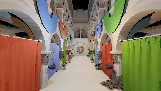
\includegraphics[width=.43\linewidth]{../../../output/screen-effects/direct.png}\hspace{4mm}
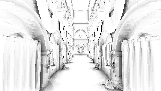
\includegraphics[width=.43\linewidth]{../../../output/screen-effects/ao-visibility.png}
\caption{同一机位。左边是给表面着色后的走廊，右边只显示 GTAO 算出的可见度，可沿拱门内圈和柱脚对照。}
\end{figure}

到了下一次绘制，\code{LightingPreview::RenderLit} 读到这份设置，组合光照时按需要调用 \code{ScreenEffects::Render}。GTAO 从逐像素的场景表面数据判断附近遮挡，再参与颜色合成。切换到单项预览时，面板可以直接显示用于观察算法的结果。用同一机位看可见度图，地面开阔处接近白，柱脚处会变暗。有了这张图，就能单独检查遮挡算得对不对，再看最终光照用的是哪份结果。

\begin{lstlisting}
uint32_t gx = (width + 7) / 8;  // (*@最右侧不足八列也分一组。@*)
uint32_t gy = (height + 7) / 8;
device.Dispatch(pipeline, resources, nullptr, gx, gy);
\end{lstlisting}
这段伪代码节选并简化了 \src{Redflag/src/Redflag/Renderer/ScreenSpace/ScreenEffects.cpp}{ScreenEffects.cpp} 中 \code{ScreenEffects::Render} 的调度。着色器按 $8\times8$ 像素分组。一幅 $17\times9$ 的图需要横向 3 组、纵向 2 组。最右和最下的一些位置落在图外，着色器先检查像素位置。传入的 \code{resources} 按着色器约定的顺序给出要读写的资源，示例的空指针表示这次没有附加的小块常量。Vulkan 实现绑定计算管线与资源，录下 \code{vkCmdDispatch}，提交后等待完成。项目当前这个同步接口返回时，后续计算或 CPU 读回能使用结果。
\readings{\src{Redflag/src/Redflag/Renderer/ScreenSpace/ScreenEffects.cpp}{ScreenEffects.cpp}\quad
\src{Redflag/src/Platform/Vulkan/VulkanComputePipeline.cpp}{VulkanComputePipeline.cpp}\quad
\href{https://docs.vulkan.org/refpages/latest/refpages/source/vkCmdDispatch.html}{Khronos · 调度工作组}}

\clearpage
\section{场景视口与鼠标坐标}
在层级里选中一盏灯，右边属性窗口会显示灯的参数。两块面板共享当前选中的实体。如果从画面中点击选取，程序还得把鼠标在窗口中的位置换算成图像中的像素。

先看这个面板是怎样出现的。\code{Begin} 和 \code{End} 标出属于一个窗口的控件，两者每帧配对。项目用 \code{IsItemHovered()} 判断鼠标是否悬停在刚创建的控件上，\code{IsItemClicked()} 则判断该控件是否被点击。在面板里，\code{ImGui::Image(texture, size)} 添加一条界面绘制记录。\code{size} 是屏幕上留给图片的宽高；增大这个尺寸会把图放大，真正增加画面细节要让引擎同时重建更多像素的输出图。

点击时，\code{GetMousePos()} 取到的是鼠标在屏幕上的位置。减去 \code{GetItemRectMin()} 返回的图像左上角，才知道点落在面板里的哪里。假设把下面这张宽 1393 像素的图缩到 696.5 个界面单位，点 A 距图像左缘 205 个单位。换回原图，横坐标便是 $205\times1393/696.5=410$。纵坐标同样换算；两者都从左上角开始数。

\begin{figure}[H]\centering
% 左图按原始宽高比显示，三个采样点以左上角为原点，单位为像素。
\begin{tikzpicture}[x=1mm,y=1mm,
  every node/.style={font=\small\sffamily,text=Ink},
  tag/.style={circle,fill=Ink,draw=white,line width=.5pt,inner sep=1.5pt,text=white,font=\sffamily\bfseries\scriptsize}]
  \node[anchor=north west,inner sep=0] at (0,0)
    {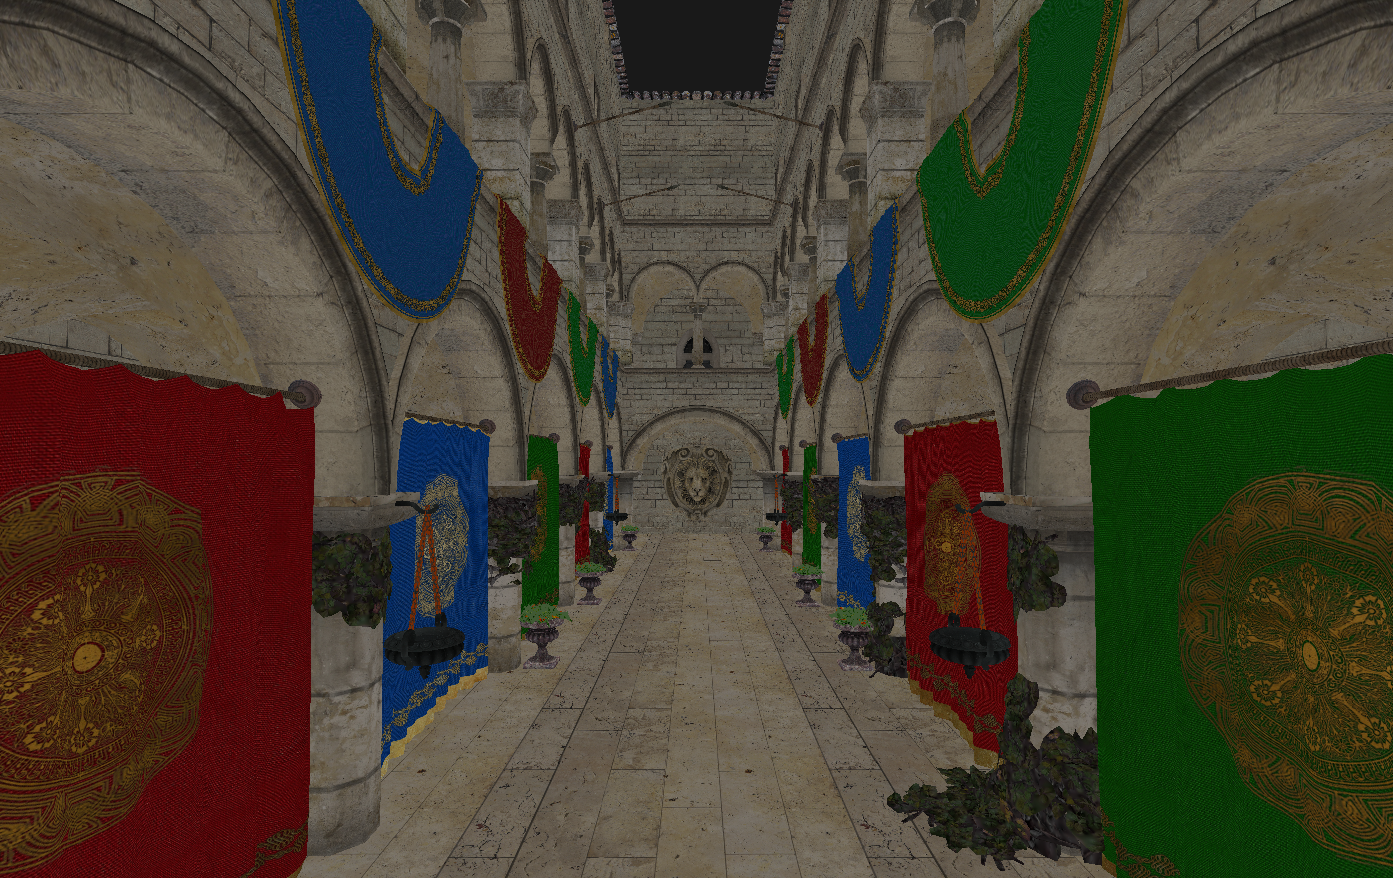
\includegraphics[width=91mm]{figures/sponza-picking.png}};
  \draw[Rule] (0,0) rectangle (91,{-91*(878/1393)});
  \foreach \x/\y/\id/\dx/\dy in {410/205/A/-6/-3,365/760/B/-7/4,690/40/C/8/-4}{
    \coordinate (sample) at ({91*((\x+0.5)/1393)},{-91*((\y+0.5)/1393)});
    \draw[Ink,line width=1.2pt] (sample)--++(\dx,\dy);
    \draw[white,line width=.55pt] (sample)--++(\dx,\dy) node[tag]{\id};
    \filldraw[fill=white,draw=Ink,line width=.45pt] (sample) circle (.75mm);
  }
  \foreach \y/\id/\what/\rgb/\value in {
    -6/A/蓝色挂毯/{29, 47, 87}/4,
    -25/B/石柱/{123, 116, 107}/4,
    -44/C/屋顶开口/{25, 25, 25}/$-1$}{
    \node[tag] at (98,\y){\id};
    \node[anchor=west,font=\sffamily\bfseries] at (102,\y){\what};
    \node[anchor=west,text=Muted] at (102,\y-5.1){RGB\enspace\rgb};
    \node[anchor=west,text=Teal] at (102,\y-10){实体编号\quad\value};
  }
\end{tikzpicture}

\caption{Sponza 中庭的底色图，白点标出取样位置。沿 A、B 看，布和石头的 RGB 相差很大，编号却相同。C 穿过屋顶开口，读到背景的 $-1$。图与读数取自同一帧的两张输出图。\href{run:../../docs/latex/source-guide/figures/SOURCES.md}{RenderDoc 第 10 帧，事件 638。}}
\end{figure}

\code{ReadPixel(410, 205)} 从同一帧取出 A 的颜色和编号。这里的 4 是本次运行中庭实体的编号；编辑器用它更新选中项，读到 $-1$ 就取消选择。面板上只需显示颜色图。Vulkan 通过 \code{ImGui\_ImplVulkan\_AddTexture} 登记这张图，返回的描述符集合供本项目作为 \code{ImTextureID} 传给 ImGui。控件的绘图数据由 \code{ImGui::Render()} 汇总。Vulkan 后端再调用 \code{ImGui\_ImplVulkan\_RenderDrawData} 把这些数据写进图形命令。最后 \code{vkQueuePresentKHR} 请求窗口系统显示这一帧。读到纹理标识时要对照当前后端；OpenGL 路径交给 ImGui 的是 OpenGL 纹理名称。
\readings{\src{RedflagForge/src/VulkanForgeLayer.cpp}{VulkanForgeLayer.cpp}\quad
\src{Redflag/src/Redflag/ImGui/VulkanImGui.cpp}{VulkanImGui.cpp}\quad
\src{Redflag/vendor/imgui/imgui.h}{项目使用的 imgui.h}\quad
\href{https://github.com/ocornut/imgui/blob/master/docs/FAQ.md}{Dear ImGui FAQ}}

\clearpage
\section{共享贴图与像素存储}
\begin{lstlisting}
auto shared = texture;           // (*@两者指向同一张贴图。@*)
frame.Textures.push_back(shared);
\end{lstlisting}
这是 \src{Redflag/src/Platform/Vulkan/VulkanDraw.cpp}{VulkanDraw.cpp} 中 \code{DrawIndexed} 的简写。这里的 \code{texture} 是共享指针。两行代码各留下一个指向同一贴图的引用。即使局部变量离开作用域，工作帧仍保存它，纹理像素也只占一份显存。这正是 \code{VulkanDraw::DrawIndexed} 将本次贴图留在工作帧中的用途。换成 \code{Scope<T>} 就不能这样复制了。它代表独占，交出所有权时用移动。面试里常见的“传引用和传值有什么区别”，在这里就是调用一次到底会不会多留下一个持有者。GPU 何时用完还由完成信号判断。

指针的拷贝很轻，整张颜色图的拷贝就不同了。每个 RGBA32F 像素包含红、绿、蓝、透明度四个 32 位浮点数，总共 16 字节。一幅宽 $W$ 的线性数组按行存放，像素 $(x,y)$ 的首字节偏移是 $16(yW+x)$。例如宽为 4 时，$(1,2)$ 的偏移是 144 字节，右边的 $(2,2)$ 紧接着就是 160 字节。\code{ComputeDevice::CreateImage} 和 \code{Readback} 的接口约定了 CPU 侧的这种排列，驱动可以另外安排 GPU 图像的内部存储。

\begin{figure}[H]\centering
\begin{tikzpicture}[x=1mm,y=1mm,
  every node/.style={font=\small\sffamily,text=Ink},labelcell/.style={font=\sffamily\footnotesize}]
  \draw[draw=Rule,rounded corners=1.4mm] (0,0) rectangle (155,50);
  \node[anchor=west,font=\sffamily\bfseries,text=Teal] at (4,44){读回内存的图像};
  \foreach \x in {0,...,3}{
    \node[labelcell] at ({22+7*\x},37.8){\x};
  }
  \node[anchor=east,labelcell,text=Muted] at (16,38){列};
  \foreach \y in {0,...,2}{
    \node[anchor=east,labelcell,text=Muted] at (16,{30-7*\y}){第 \y 行};
    \foreach \x in {0,...,3}
      \draw[fill=Soft,draw=Rule] ({18.5+7*\x},{26.5-7*\y}) rectangle ++(7,7);
  }
  \filldraw[fill=Teal,draw=Teal] (25.5,12.5) rectangle ++(7,7);
  \filldraw[fill=Rust,draw=Rust] (32.5,12.5) rectangle ++(7,7);
  \node[text=white,labelcell] at (29,16){A};
  \node[text=white,labelcell] at (36,16){B};
  \draw[Rule] (51,7)--(51,42);
  \node[anchor=west,font=\sffamily\bfseries,text=Teal] at (56,44){第 2 行展开后};
  \foreach \x/\lo/\hi/\bg/\fg in {57/128/143/Soft/Ink,80/144/159/Teal/white,103/160/175/Rust/white,126/176/191/Soft/Ink}{
    \draw[fill=\bg,draw=Rule] (\x,20) rectangle ++(23,12);
    \node[labelcell,text=\fg] at ({\x+11.5},26){\lo--\hi};
  }
  \node[text=Teal,font=\sffamily\bfseries] at (91.5,36){A};
  \node[text=Rust,font=\sffamily\bfseries] at (114.5,36){B};
  \node[anchor=west,text=Muted] at (56,13){数字是距整张图开头的字节数。};
  \node[anchor=west,text=Muted] at (56,7){每格一个像素，依次放 R、G、B、A。};
\end{tikzpicture}

\caption{以每行 4 个 RGBA32F 像素为例。跳过两行共 $2\times4\times16=128$ 字节；再向右一个像素，A 正好从第 144 字节开始。B 紧跟在 A 的四个颜色分量之后。}
\end{figure}

沿一行像素往右读，下一项紧挨着刚读过的地址。这种访问方式有空间局部性。一段时间里反复拿同一组三角形求交，又会多次用到刚读过的数据，这叫时间局部性。CS:APP 第六章用数组访问来讲这两个概念。计算缓冲实际落在系统内存还是显卡本地内存则要看 Vulkan 报告的内存类型。项目在同一中庭、同一画幅上测了两种放置方式，原始时间与条件见\href{run:Redflag-Rendering-Performance.pdf}{《渲染性能实测》}。

\href{run:../api/index.html}{离线 API 手册}可按 \code{CreateBuffer}、\code{ReadPixel}、\code{SetCamera} 等名字检索重载和参数。读源文件时先看谁创建对象，再看一帧里谁引用它；最后到工作帧或退出路径确认它最后一次被使用的时刻。
\readings{\href{https://www.informit.com/content/images/9780321714114/samplepages/0321714113.pdf}{《C++ Primer》第五版 · 动态内存}\quad
\href{https://csapp.cs.cmu.edu/3e/pieces/preface3e.pdf}{CS:APP 第三版 · 第 6 章目录}\quad
\href{https://csapp.cs.cmu.edu/3e/labs.html}{作者的 Cache Lab}\quad
\href{run:Redflag-RHI-Vulkan-Plan.pdf}{架构册 · 贴图的持有与释放}}
\clearpage
\section{石柱的表面与光照}
神庙的石柱底色很浅，背光的一面却是深灰。要算出这层差别，先得知道镜头看见的是哪块石头，再查它的颜色和朝向。三角形投影到屏幕后，覆盖的采样位置会产生片元，这一步叫光栅化。深度测试留下最近、也通过材质透明度裁剪的一层。

\begin{figure}[H]\centering
\begin{minipage}[t]{.483\linewidth}\centering
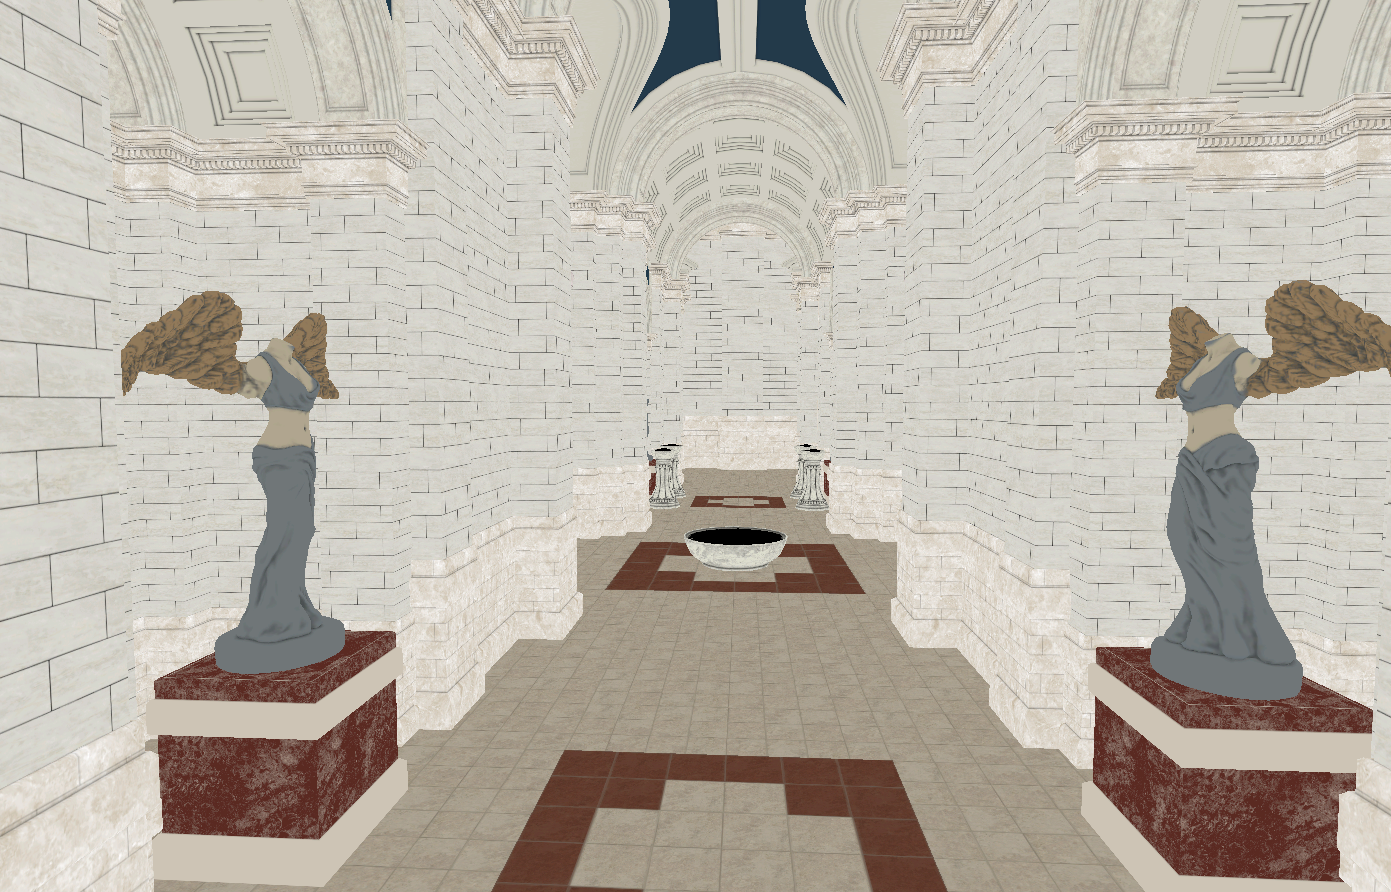
\includegraphics[width=\linewidth]{../../../output/scenes/sun-temple/albedo.png}\\
{\sffamily\small 材质的底色}
\end{minipage}\hfill
\begin{minipage}[t]{.483\linewidth}\centering
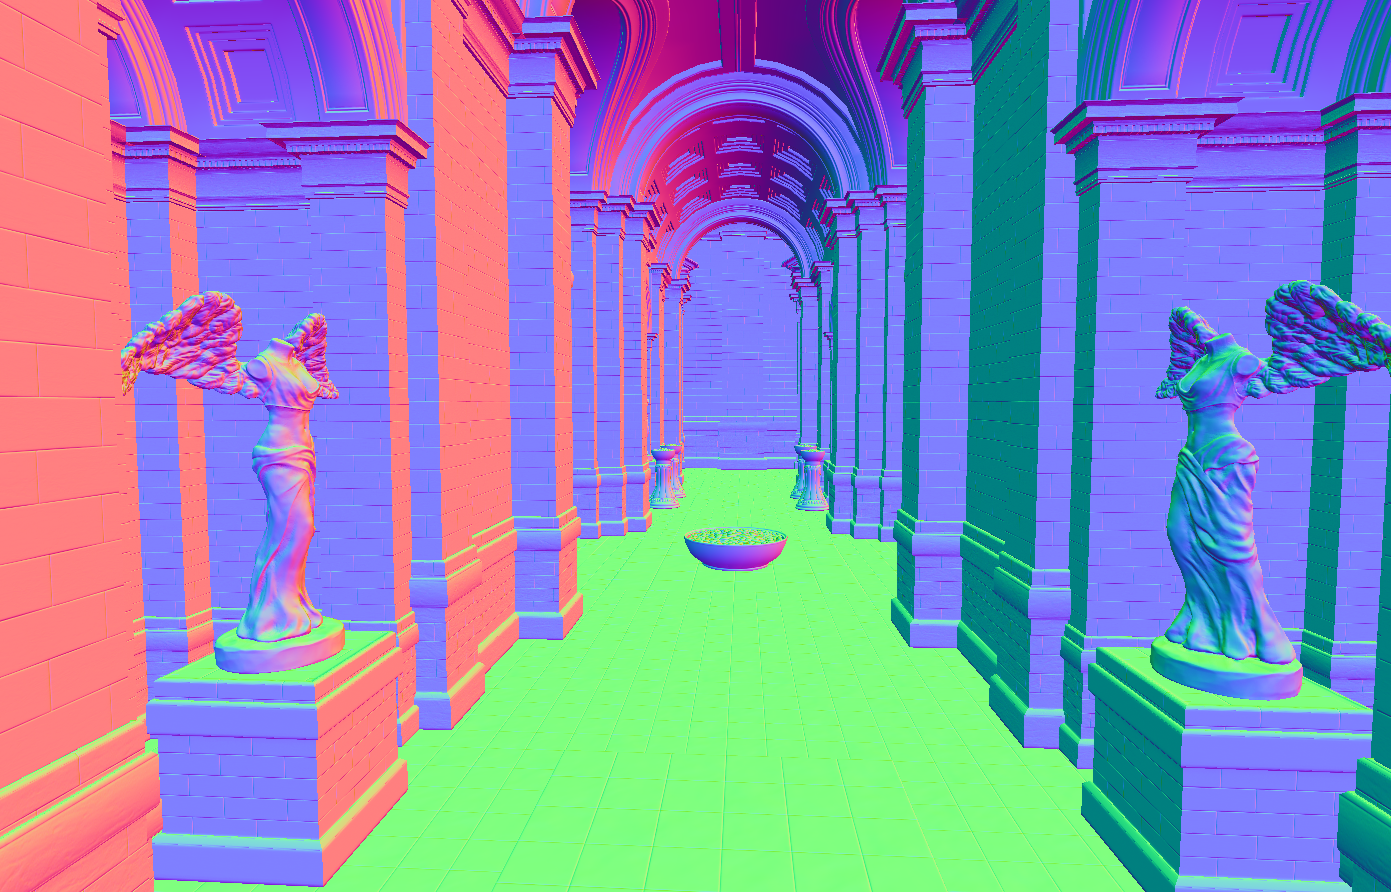
\includegraphics[width=\linewidth]{../../../output/scenes/sun-temple/normal-depth.png}\\
{\sffamily\small 世界坐标中的法线}
\end{minipage}
\caption{同一次绘制的两个输出。左图的石块之间只有细微色差；在右图，面向镜头的墙接近蓝色、向上的地面是绿色，墙上斜切的线脚又有其他颜色。右图以 RGB 标出法线的 $x,y,z$ 三个分量，深度在第四个分量中。}
\end{figure}

\begin{figure}[H]\centering
\begin{tikzpicture}[x=1mm,y=1mm,every node/.style={font=\sffamily\small,text=Ink},
    station/.style={draw=Rule,rounded corners=1.2mm,align=center,inner sep=2.4mm},
    arrow/.style={-{Stealth[length=2mm]},draw=Teal,line width=.75pt}]
  \draw[draw=Rule,rounded corners=1.4mm] (0,0) rectangle (155,34);
  \node[station,fill=Soft] (raster) at (25,17) {\texttt{Mesh.frag}\\底色、法线与深度};
  \node[station,fill=warm] (pack) at (79,17) {\texttt{PackSurfaces.comp}\\还原每个位置};
  \node[station,fill=pale] (lit) at (134,17) {\texttt{RenderLit}\\直接光与间接光};
  \draw[arrow] (raster)--(pack);
  \draw[arrow] (pack)--(lit);
\end{tikzpicture}
\caption{箭头沿着显存中的数据走。左段读取同一帧的两张图，中段写入包含位置、法线和底色的 \code{GISurface} 数组，右段按像素使用它。}
\end{figure}

从相机看到的深度仍是投影之后的数。比如图像正中的石壁，深度是 $0.99738$。要照亮它，还需要知道它离场景中的点光源有多远。\code{PackSurfaces.comp} 取出这个深度，按 $2d-1$ 换回引擎相机使用的范围，与像素中心的横、纵坐标组成四维向量。乘以本次相机矩阵的逆，再除以结果的 $w$，得到石壁在世界中的位置。这次投影若有 TAA 的采样偏移，还原时也使用同一次偏移。

镜头看见的第一层由光栅绘制取得。计算阴影和间接光时，着色器还要查询离开这一层的光线会撞上哪个三角形。两段工作通过显存交换数据，当前实现会等待每段提交完成。图中模型为 Epic Games 的 Sun Temple，项目的布光与衍生截图沿用 CC BY-NC-SA 4.0 许可。

\readings{\src{Redflag/src/Platform/Vulkan/Shaders/Mesh.frag}{Mesh.frag}\quad
\src{Redflag/src/Platform/Vulkan/Shaders/PackSurfaces.comp}{PackSurfaces.comp}\quad
\href{run:../scenes/sun-temple/capture.json}{RenderDoc 帧与像素}\quad
\href{https://developer.nvidia.com/ue4-sun-temple}{NVIDIA ORCA 原场景}\\
\href{https://www.cs.cornell.edu/courses/cs4620/2018fa/slides/10rasterization.pdf}{虎书作者 Marschner · 光栅化讲义，第 3 页}}

\clearpage
\section{两块玻璃的颜色与折射}
打开项目面板里的 \path{Glass-Studio.redflag}，墙前立着两片玻璃。在属性中选「青色玻璃」的材质，将折射率从 1 改为 1.5。墙条在玻璃外保持原位，穿过边缘后却向旁边错开。下图保留了墙条在玻璃上方的一小段，可以直接沿同一条边看下来。

\begin{figure}[H]\centering
\begin{minipage}[t]{.48\linewidth}\centering

\includegraphics[width=\linewidth]{../../../output/scenes/glass-studio/straight-detail.png}\\
{\small 折射率 1.0}
\end{minipage}\hfill
\begin{minipage}[t]{.48\linewidth}\centering

\includegraphics[width=\linewidth]{../../../output/scenes/glass-studio/bent-detail.png}\\
{\small 折射率 1.5}
\end{minipage}
\caption{演示时两块玻璃同时改动。图为 Vulkan 编辑器两次运行的第 12 帧、同一位置的裁剪。左图的墙条变了颜色，右图的墙条在边缘处还发生位移。\href{run:../scenes/glass-studio/bent.png}{完整视口图}}
\end{figure}

先看颜色。一个像素若同时落在两块玻璃上，琥珀色玻璃的不透明度是 0.30，青色是 0.24。第一层剩下 $1-0.30=0.70$ 的背景，第二层又留下其中的 $0.76$，最后约有 $53.2\%$ 的背景颜色。引擎用两个数的对数之和保存这个乘积，合成时取指数就能还原。两种玻璃各自贡献多少颜色，则按不透明度和深度加权平均。这样几何可以直接按场景中的次序提交；当颜色差异很大且紧密交叠时，这个平均值是近似。

再看墙条的位置。把玻璃面的垂直方向叫作法线，入射角和折射角均从它量起。空气的折射率近似为 1，玻璃取 1.5。斯涅尔定律给出 $1\sin\theta_i=1.5\sin\theta_t$。若入射角为 $30^\circ$，折射角约为 $19.5^\circ$，光线在玻璃中向法线靠拢。\code{CompositeTransparency.comp} 的 \code{main} 用 \code{refract} 得到这个方向，再按材质给出的世界单位厚度，求光线到达另一面的地点。把这个点投回屏幕，就知道该去墙面图的哪里读颜色。落在屏幕外时，保留原处背景；落在玻璃前方的遮挡物上，对应的采样点也沿原方向取色。

这张墙面图已经算完直接光、间接光以及开启的反射和雾。两片玻璃重叠时，合成只使用一组加权的方向和厚度，因此无法还原光线多次进出玻璃的路线。用两次回放的完整图逐点比较，在 $1{,}243{,}949$ 个像素中，$157{,}890$ 个至少有一个显示颜色通道变化超过 $8/255$。这是这个场景的画面差异；验证绘制顺序则另用两片测试网格，调换顺序后读回的最大颜色差为 0。

\readings{\src{Redflag/src/Platform/Vulkan/Shaders/Mesh.frag}{Mesh.frag · main}\quad
\src{Redflag/src/Platform/Vulkan/Shaders/CompositeTransparency.comp}{CompositeTransparency.comp · main}\quad
\href{run:../scenes/glass-studio/capture.json}{帧、事件与像素}\\
\href{https://learnopengl.com/Advanced-OpenGL/Blending}{LearnOpenGL · 透明度}\quad
\href{https://jcgt.org/published/0002/02/09/}{McGuire 与 Bavoil · 加权混合}\quad
\href{https://pbr-book.org/4ed/Reflection_Models/Specular_Reflection_and_Transmission}{PBRT 第四版 §9.3 · 折射}}

\clearpage
\section{材质贴图的绿色与蓝色通道}
色板只有两个三角形。看左上角的红格，底色贴图把它涂成红色，另一张贴图决定它反光时的样子。glTF 将粗糙度放在这张材质贴图的绿色通道，将金属度放在蓝色通道。粗糙度越大，高光通常铺得越开。金属度为零对应塑料一类的绝缘体，为一对应金属。两项都是 $0$ 到 $1$ 之间的比例。

\begin{figure}[H]\centering
\newcommand{\channelsample}[1]{%
  \begin{tikzpicture}
    \node[anchor=south west,inner sep=0] (photo) at (0,0) {%
      \includegraphics[width=\linewidth,trim=183bp 37bp 183bp 37bp,clip]{../../../output/profiling/material-channels/#1.png}};
    \begin{scope}[x={(photo.south east)},y={(photo.north west)}]
      \draw[black,line width=1.55pt] (.295,.703) circle[radius=2pt];
      \draw[white,line width=.8pt] (.295,.703) circle[radius=2pt];
    \end{scope}
  \end{tikzpicture}}
\begin{minipage}[t]{.31\linewidth}\centering
\channelsample{albedo}\\[-1pt]
{\small\sffamily 底色}
\end{minipage}\hfill
\begin{minipage}[t]{.31\linewidth}\centering
\channelsample{roughness}\\[-1pt]
{\small\sffamily 粗糙度}
\end{minipage}\hfill
\begin{minipage}[t]{.31\linewidth}\centering
\channelsample{metallic}\\[-1pt]
{\small\sffamily 金属度}
\end{minipage}
\caption{RedflagForge 材质色板，RenderDoc 第 12 帧。圆圈标出同一个像素。从左向右看，它的底色偏红、粗糙度较低、金属度较高。后两张直接用灰度表示数值，越亮数值越大。}
\end{figure}

在材质贴图的同一位置，绿色通道存着 64，蓝色通道存着 255。两个数各占一个字节，除以 255 就能换成 $0$ 到 $1$ 的比例。模型文件给整块色板指定了粗糙度系数 $0.8$、金属度系数 $0.6$。将各自的系数乘进去，就能算出着色器应该读到什么。
\[
  \text{粗糙度}=0.8\,\frac{64}{255}\approx0.200784,\qquad
  \text{金属度}=0.6\,\frac{255}{255}=0.6 .
\]

\codewhere{着色器节选}{Redflag/src/Platform/Vulkan/Shaders/Mesh.frag}{main}
\begin{lstlisting}
vec2 material = unpackUnorm2x16(u_Object.MaterialFactors);
if ((u_Object.MaterialFlags & 4u) != 0u)  // (*@当前材质有这张贴图。@*)
    material *= texture(u_MetallicRoughnessMap, v_TexCoord).bg;
\end{lstlisting}

第一行取出本次绘制的两个系数。代码把金属度排在前面，所以 \code{.bg} 依次取蓝、绿通道。没有贴图时直接用系数。本页截帧时由着色器将底色从 sRGB 换为线性亮度，现版由 Vulkan 的 sRGB 纹理格式完成，末位精度可能不同。两版都按线性比例读取粗糙度和金属度。

在原图坐标 $(311,167)$ 读到粗糙度 $0.200733$，与手算相差约 $0.000052$。绘制时，两项材质各用 12 位保存，从 0 到 1 有 4095 个间隔，四舍五入最多差半个间隔，约 $0.000122$。这一点差别落在舍入误差之内。
\readings{\href{https://registry.khronos.org/glTF/specs/2.0/glTF-2.0.html\#metallic-roughness-material}{Khronos · glTF 2.0 §3.9.2}\quad
\src{Redflag/src/Platform/Vulkan/Shaders/MaterialChannels.glsl}{MaterialChannels.glsl · encodeMaterial}\quad
\href{run:../profiling/material-channels/samples.json}{四格原始读数}}

\clearpage
\section{色板上的法线}
色板第一次画出来时，中间有一条黑带。左上红格的粗糙度和金属度已经对上了，接着可以检查光照用到的方向。色板平放在 $xy$ 平面，正面朝向镜头，法线应沿 $+z$。从 RenderDoc 的绘制事件 27 读第二张输出图，却发现整个色板都沿 $+y$，像是把平面立错了方向。

\begin{figure}[H]\centering
\begin{minipage}[t]{.483\linewidth}\centering

\includegraphics[width=.68\linewidth,trim=183bp 37bp 183bp 37bp,clip]{../../../output/profiling/material-channels/panel-before.png}\hfill
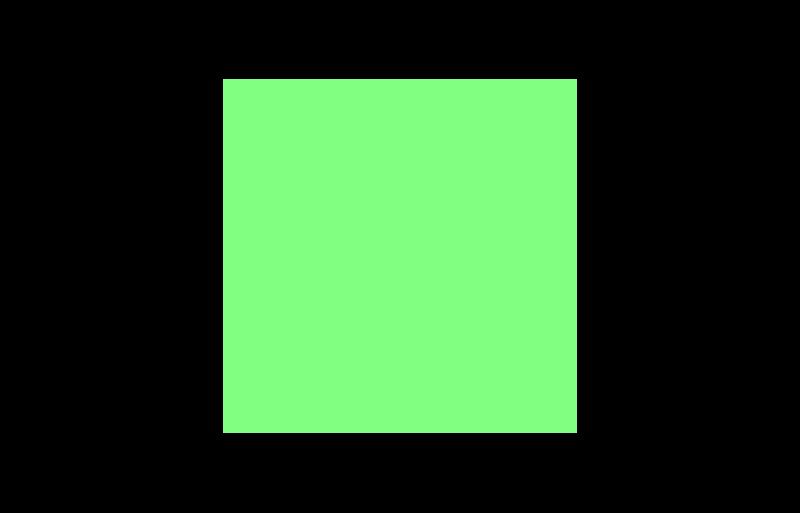
\includegraphics[width=.29\linewidth,trim=183bp 37bp 183bp 37bp,clip]{../../../output/profiling/material-channels/normal-before.png}\\
{\small\sffamily 修正前\quad 法线 $(0,1,0)$}
\end{minipage}\hfill
\begin{minipage}[t]{.483\linewidth}\centering
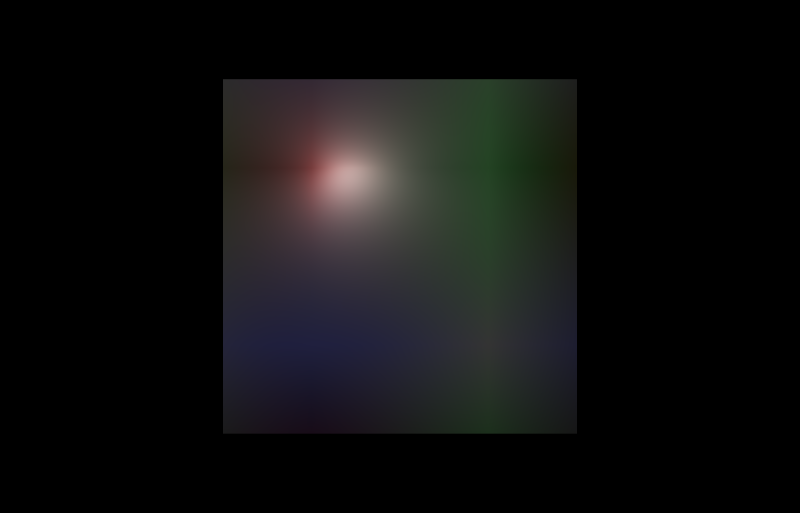
\includegraphics[width=.68\linewidth,trim=183bp 37bp 183bp 37bp,clip]{../../../output/profiling/material-channels/panel.png}\hfill
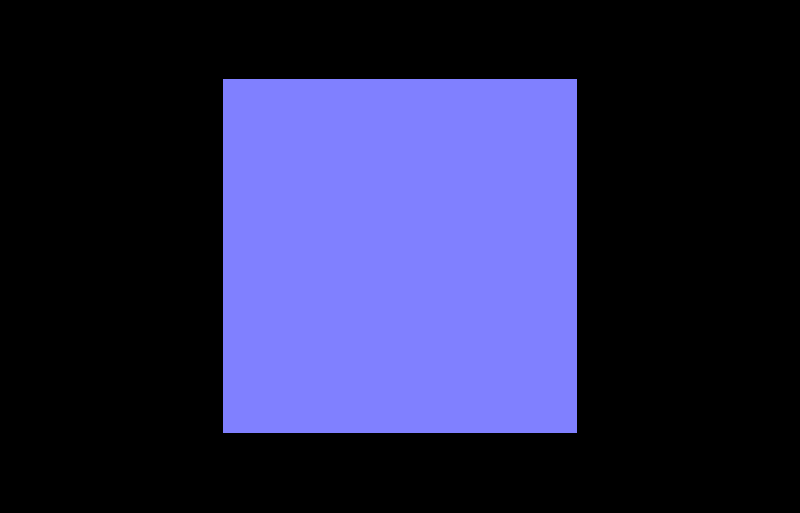
\includegraphics[width=.29\linewidth,trim=183bp 37bp 183bp 37bp,clip]{../../../output/profiling/material-channels/normal-after.png}\\
{\small\sffamily 修正后\quad 法线 $(0,0,1)$}
\end{minipage}
\caption{同机位两次 RenderDoc 回放。每组大图是场景面板，小图把世界法线的 $x,y,z$ 分别画成红、绿、蓝。修正后，高光出现在点光源照向的左上区域。两帧均覆盖 125,316 个模型像素。}
\end{figure}

色板文件给了顶点位置，省略了法线。取第一个三角形，从同一顶点沿两条边走，模型局部坐标中的边向量是 $(0,-4,0)$ 和 $(4,0,0)$。它们叉乘得到 $(0,0,16)$，除以长度 16 就是单位法线 $(0,0,1)$。glTF 约定缺少法线时按面计算，\code{Model::Load} 也已请求 \code{aiProcess\_GenNormals}。问题出在编译 Assimp 时关闭了这个步骤，模型最终读到了默认的朝上方向。

\codewhere{构建配置节选}{premake5.lua}{assimp}
\begin{lstlisting}
removedefines { "ASSIMP_BUILD_NO_GENFACENORMALS_PROCESS" }
files { "Redflag/vendor/assimp/code/GenFaceNormalsProcess.cpp" }
\end{lstlisting}

第一行解除对面法线生成器的禁用，第二行把它的实现编入项目。重新导入后，还可以用模型回归测试读取实际上传的三个顶点，分别检查法线是否等于预期方向。

回到同一帧，事件 39 将每个像素交给光照计算。一个表面用位置、法线和底色三个四分量向量保存，每个向量 16 字节，共 48 字节。位置的第四项标记这里有模型，法线的第四项保存粗糙度，底色的第四项保存金属度。在事件 27 还能查到整次绘制共用的压入常量（push constants）。拾取时存实体编号的 4 个字节，在材质绘制时存两个 16 位系数，因此整块仍为 128 字节。
\readings{\src{Redflag/src/Platform/Vulkan/Shaders/PackSurfaces.comp}{PackSurfaces.comp · main}\quad
\src{Redflag/src/Platform/Vulkan/VulkanDraw.cpp}{VulkanDraw.cpp · DrawIndexed}\quad
\href{run:../profiling/material-channels/README.md}{两份原帧与命令}\\
\href{https://registry.khronos.org/glTF/specs/2.0/glTF-2.0.html\#meshes}{glTF 2.0 §3.7.2.1 · 几何属性}\quad
\href{https://pbr-book.org/4ed/Shapes/Triangle_Meshes}{PBRT 第四版 §6.5 · 三角形网格}}

\clearpage
\section{摄影棚的环境反射}
转动一台金属相机，即使棚灯没有出现在取景框里，镜圈上仍能映出灯的轮廓。要画出这条亮边，可以把站在物体旁边向四周拍到的光记录在一张全景图上。HDR 图还能保留比白纸亮得多的光源。画镜圈时，程序先从像素所在的表面位置求出看向观察者的方向 $V$，再取该处的法线 $N$。两者都是单位向量。视线从观察者沿 $-V$ 射向镜面，反射后的方向为
\[
  R=2(N\mathbin{\cdot}V)N-V .
\]
正对镜面看时 $V=N$，于是 $R=N$，应当查镜面正前方的环境。斜着看时，观察方向沿表面的分量会反向，亮窗便移到倒影里的另一个位置。

\begin{figure}[H]\centering
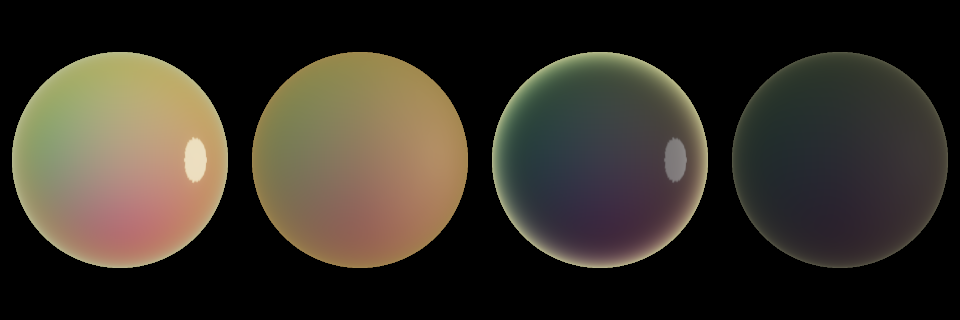
\includegraphics[width=.89\linewidth]{../../../output/profiling/environment-lighting/material-spheres.png}
\caption{Redflag 的 Vulkan 着色器绘制的镜面反射。四个球依次为光滑金属、粗糙金属、光滑涂漆、粗糙涂漆，使用同一张带亮窗的测试全景。球的形状和底色相同。}
\end{figure}

光滑表面主要映出 $R$ 附近很小一片天空。粗糙表面有许多朝向稍有不同的小面，同一条视线会收到更大一片环境的光。从左向右看图中前两颗球，亮窗的轮廓展开，最亮处也变暗了。我们可以预先把不同方向附近的光做加权平均，保存五层倒影。第 0 层保留细节，第 4 层反射范围最宽。粗糙度为 $0.375$ 时，着色器取第 $4\times0.375=1.5$ 层，即把第 1、2 层各取一半。五层是本项目的存储选择。

环境给出了光从哪里来，还要估计表面把多少光反射回来。光正对空气和普通玻璃的交界面时，按折射率 $1$ 与 $1.5$ 计算，反射比例约为 $((1.5-1)/(1.5+1))^2=0.04$。这里把它作为普通非金属的起点。纯金属则用材质底色描述正面反射的颜色。实现根据观察角度和粗糙度查一张预先积分的二维表。表里有两个系数，用来把环境的颜色换算成表面朝观察者反射的亮度。
\readings{\href{https://www.pbr-book.org/4ed/Reflection_Models/Roughness_Using_Microfacet_Theory}{PBRT 第四版 §9.6，微表面}\quad\href{https://learnopengl.com/PBR/IBL/Specular-IBL}{LearnOpenGL，Specular IBL}\quad\src{Redflag/src/Redflag/Renderer/ScreenSpace/Shaders/Environment.glsl}{Environment.glsl}}

\clearpage
\section{屏幕内外的倒影}
摄影棚的机身右侧有一道窄边。固定镜头和灯，只切换“镜面 IBL”，两张图里这道边受到的光便有明显差别。底色、法线和两项材质参数来自同一件模型。两次截帧中用于照明的底色和材质图逐像素相同。

\newcommand{\studioview}[2]{\begin{minipage}{.485\linewidth}\centering
\begin{tikzpicture}
  \node[inner sep=0,anchor=south west] (shot) at (0,0) {\includegraphics[width=\linewidth]{../../../output/profiling/material-studio/#1.png}};
  \begin{scope}[x={(shot.south east)},y={(shot.north west)}]
    \draw[white,line width=.9pt] (.6556,.5702) circle[radius=1.6mm];
    \draw[black,line width=.25pt] (.6556,.5702) circle[radius=1.8mm];
  \end{scope}
\end{tikzpicture}\\\small #2\end{minipage}}
\begin{figure}[H]\centering
\studioview{no-ibl}{关闭镜面 IBL}\hfill\studioview{after}{开启镜面 IBL}
\caption{Khronos 示例 Antique Camera 和 Poly Haven 全景 Studio Small 09。白圈中心是机身边框上的像素 $(524,220)$。取它周围 $5\times5$ 个像素，在显示变换前读回线性红通道，平均值从 0.00524 升到 0.24281。}
\end{figure}

在组合光照中，\code{LightingPreview::RenderLit} 先准备直接光和漫反射的颜色。若场景选了环境图，就可以再加上镜面看到的环境。打开屏幕空间反射（SSR）后，反射光线有时会先碰到画面里的一堵墙。这时应该用墙的颜色。走出屏幕或找不到合适的交点时，环境仍能提供来自该方向的光。下面是两条路在着色器里的简写。

\begin{lstlisting}
// (*@伪代码。surfaceLighting 已包含直接光和间接漫反射。@*)
vec3 reflected = sampleEnvironment(R, roughness);
if (screenRayHitsWall)
    reflected = sampleWallLight() * reflectionWeight;
return surfaceLighting + reflected;
\end{lstlisting}
\noindent{\small 着色器见 \src{Redflag/src/Redflag/Renderer/ScreenSpace/Shaders/StochasticSSR.comp}{StochasticSSR.comp} 的 \code{main}。它调用 \code{specularEnvironment} 时，已经计入材质的反射比例。}

可以摆两片金属和一堵绿墙来检查。第一片能从屏幕里找到绿墙，开关镜面 IBL，像素的四个分量都相同。第二片向画外反射，开启后测得线性 RGB 为 $(1.717,0.511,0.120)$。这个实验能发现同一处倒影被加亮两次的问题。全景只记录了从一个位置看到的房间，若要还原紧靠物体、又藏在取景框外的遮挡，还需要该物体附近的几何信息。
\readings{\src{output/profiling/environment-lighting/README.md}{绿墙与画外反射的截帧}\quad\src{output/profiling/material-studio/measurements.json}{摄影棚的亮度读数}\quad\href{https://polyhaven.com/a/studio_small_09}{Sergej Majboroda，Studio Small 09}}

\clearpage
\section{灯牌的颜色与亮度}
关掉房间里的灯，仍能看见亮着的灯牌。看一块普通木板，眼睛收到的是木板反射过来的光；换成灯牌，表面还会自己发光。在灯牌上的某一点，朝眼睛送出的光 $L_o$ 就是这两份光之和，$L_o=L_r+L_e$。其中 $L_r$ 表示反射光，$L_e$ 表示表面自身发出的光。点光源的阴影可以遮住照向灯牌的光，灯牌上通电的笔画仍然亮着。渲染时先把这两项在线性空间相加，之后才按相机曝光把亮度换成屏幕颜色。

\begin{figure}[H]\centering
\begin{minipage}[b]{.46\linewidth}\centering
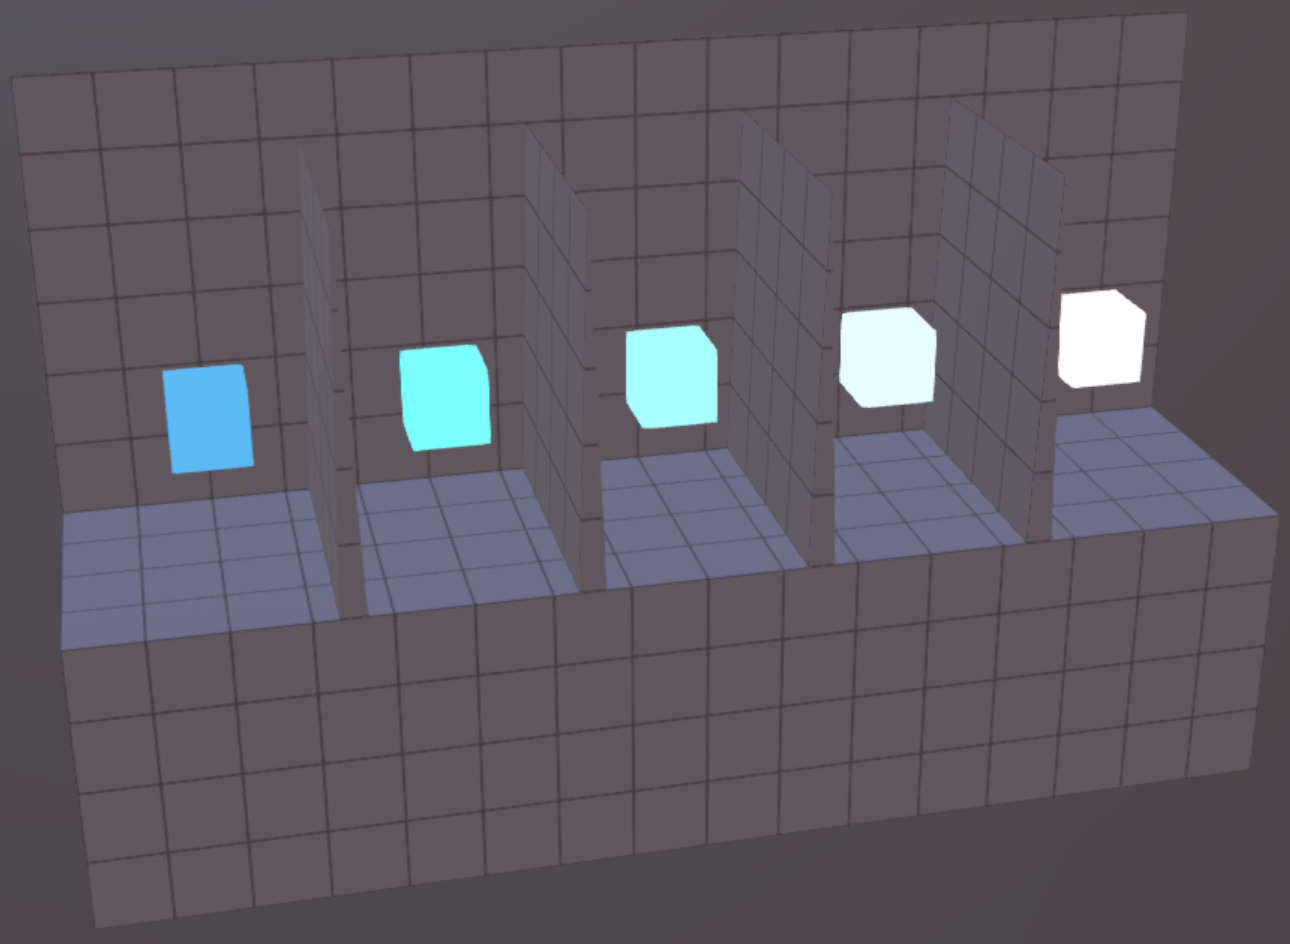
\includegraphics[height=46mm]{figures/emissive-strength-reference.jpg}\\[-1pt]
{\small\sffamily glTF 强度示例}
\end{minipage}\hfill
\begin{minipage}[b]{.51\linewidth}\centering

\includegraphics[height=46mm]{../../../output/profiling/emissive-studio/wide.png}\\[-1pt]
{\small\sffamily Redflag 灯光实验室}
\end{minipage}
\caption{左图五个立方体使用相同的颜色，从左往右将发光强度设为 1、2、4、8、16。原图由 Ed Mackey（AGI，2022）用 BabylonJS 绘制，\href{https://creativecommons.org/licenses/by/4.0/}{CC BY 4.0}。右图来自项目 Vulkan 编辑器的 RenderDoc 回放，三条橙色色带属于同一件材质，中间一条在发光贴图上更暗。}
\end{figure}

右图的材质在 glTF 文件中写着发光因子 $(1,\,0.12,\,0.035)$ 和强度 4。模型导入时把两者相乘，得到材质的 \code{Emission}，即 $(4,\,0.48,\,0.14)$。贴图再控制灯牌的哪些地方亮。白色像素的三个通道都写作 255，乘数是 1；黑色像素的乘数为 0。灰色的 128 在 sRGB 中表示的线性亮度约为 $((128/255+0.055)/1.055)^{2.4}=0.21586$。因此灰带红通道应当是 $4\times0.21586\approx0.86344$，同一配色的 Vulkan 像素测试读到 0.86328。它是曝光前的相对亮度，可以超过 1。

\codewhere{片元着色器节选}{RedflagForge/assets/shaders/Renderer3D_Mesh.glsl}{main}
\begin{lstlisting}
if (u_UseEmissiveMap != 0)
    emission *= texture(u_EmissiveMap, v_EmissiveUV).rgb;
// (*@把这一点自己发出的光加在反射光上。@*)
vec3 color = ambient + Lo + emission;
\end{lstlisting}

没有发光图，整块表面就按材质的发光颜色来画。没有填写发光因子，glTF 默认给黑色。材质的底色和自发光可以分别设定，发光图的透明通道也不会把模型上的笔画挖掉。
\readings{\href{https://github.com/KhronosGroup/glTF-Sample-Assets/tree/main/Models/EmissiveStrengthTest}{Khronos 示例库 · 左图与模型}\quad
\href{https://registry.khronos.org/glTF/specs/2.0/glTF-2.0.html\#additional-textures}{glTF 2.0 §3.9.3}\quad
\href{https://github.com/KhronosGroup/glTF/tree/main/extensions/2.0/Khronos/KHR_materials_emissive_strength}{自发光强度扩展}}

\clearpage
\section{灯牌照到的墙面}
OpenGL 在画灯牌时就知道表面反射了多少光，上一页的加法直接写进场景颜色即可。画许多块灯牌时，同一张贴图可以只选一次，各实例仍各自带一份发光颜色。项目测试摆了四块灯牌，前两块共用网格和贴图，后两块分别没有贴图和使用绿色贴图。实际用了三次主绘制。没有贴图的那块在红通道读到 4，绿色的那块在绿通道读到 2.5，鼠标拾取仍能分辨四块牌子。

Vulkan 编辑器先为每个可见像素记下表面位置、法线和材质，随后才算各处分到了多少光。这 48 字节的数据已经有了各自的用途。遇到实心发光材质时，编辑器另画一张发光图，再把它加进计算好的场景颜色。记录灯牌这次绘制时，原来传底色的三个数可以改传发光颜色，每次绘制的压入常量仍为 128 字节。挡在灯牌前面的物体也参与深度判定，墙后面的灯牌不会盖到墙面上。玻璃则随透明表面按覆盖率合成。

\codewhere{调用节选}{Redflag/src/Platform/Vulkan/Shaders/Emission.frag}{main}
\begin{lstlisting}
// (*@颜色随这次绘制传入；贴图取当前位置的发光图案。@*)
emission.rgb = u_Object.Color.rgb * texture(emissiveMap, v_EmissiveUV).rgb;
\end{lstlisting}

\begin{figure}[H]\centering
\begin{minipage}[b]{.455\linewidth}\centering

\includegraphics[width=\linewidth]{../../../output/profiling/emissive-studio/wall.png}\\[-1pt]
{\small\sffamily 灯牌开启，墙面红通道 0.09709}
\end{minipage}\hspace{4mm}
\begin{minipage}[b]{.455\linewidth}\centering

\includegraphics[width=\linewidth]{../../../output/profiling/emissive-studio/wall-off.png}\\[-1pt]
{\small\sffamily 灯牌关闭，墙面红通道 0}
\end{minipage}
\caption{灯光实验室的两次正式 Vulkan 截帧。从同一位置看白墙，灯牌的四个角都已移出画面。这个场景没有点光源，关掉灯牌以后，白墙就暗了下来。数字取自第 24 帧，在图上距左边 282 像素、距顶边 186 像素处周围 $5\times5$ 个像素取平均。\href{run:../profiling/emissive-studio/frames.json}{原帧与设置}。}
\end{figure}

这时屏幕上的发光图已经看不到灯牌。要把墙照亮，计算间接光的光线仍要能命中镜头外的灯牌。命中一个三角形后，\code{raySurface} 用其三个顶点的贴图坐标插出击中位置的坐标，从发光图取出这一点的颜色。\code{incomingAt} 将它与这块表面反射的光相加。DDGI 把从各方向收到的光存到探针，之后墙面就能查到旁边灯牌送来的光。另用 $17\times17$ 像素测试一面墙，直接对矩形灯牌做面积积分，墙面线性红通道的均值为 0.21522，ReSTIR GI 累积 512 帧后得到 0.21396。

\readings{\src{Redflag/src/Redflag/Renderer/GI/Shaders/GI.comp}{GI.comp · raySurface 与 incomingAt}\quad
\href{run:../profiling/emissive-material/README.md}{显卡读数与像素位置}\\
\href{https://pbr-book.org/4ed/Light_Sources/Area_Lights}{PBRT 第四版 §12.4 · 面光源}\quad
\href{run:../profiling/emissive-gi/measurements.csv}{墙面参考积分与 GPU 实测}}

\clearpage
\section{镂空材质的着色器接口}
给编辑器中已有的立方体换一张带孔的贴图，只需要设置材质。下例中的 \code{image} 是用 \code{Texture2D::Create(path)} 读入的 RGBA 图片，A 通道在孔内为 0，在实心处为 1。材质和场景组件保留对贴图的共享引用，绘制这只立方体时可以一直使用它。

\begin{lstlisting}
// (*@调用示例。接口见 Material.h、Components.h。@*)
void SetFence(MeshRendererComponent& cube, const Ref<Texture2D>& image)
{
    Ref<Material> material = Material::Create(image);
    material->Alpha = AlphaMode::Mask;
    material->AlphaCutoff = 0.5f;  // (*@等于 0.5 的位置也保留。@*)
    cube.Mat = material;
}
\end{lstlisting}

接下来是引擎的工作。\code{SceneRenderer::DrawGeometry} 从组件取出材质，把底色贴图传给 \code{CommandList::DrawIndexed}。其他会影响表面的参数装在 \code{SurfaceMaterial} 里，其中 \code{AlphaCutoff} 给出保留像素所需的透明度，\code{Opacity} 可以再放一张单独的透明图。没有提供透明图时，Vulkan 后端绑定一张白图，读出来的值为 1，对乘积没有影响。

普通绘制与鼠标拾取按三角形上的贴图坐标读取这两张图。底色图的 A、单独透明图的 R 和此次绘制的透明度相乘，小于裁剪值就留下一个孔。后面的模型仍可写下自己的颜色、深度与实体编号。\code{Mesh.frag} 负责主绘制，\code{Emission.frag} 单独画材质发出的光，两者调用同一个 \code{coversSample}。打开 SSAA 时，光照绘制会在一个像素里区分四个位置。

间接光要找的是一条射线碰到的表面。\code{CollectModels} 因此把材质的透明度和裁剪值交给光照计算，模型加载器从模型内嵌图片或指定的贴图文件取像素。\code{AlphaMask.glsl} 在每个可能的交点调用 \code{passesAlphaMask}，穿过孔后继续检查更远的三角形。若在内存里生成一张新贴图，光照加载器目前无法从文件重建它的透明度。需要同时得到正确的相机画面、阴影和烘焙时，请使用有文件来源的贴图。

\readings{\src{Redflag/src/Redflag/Renderer/RHI/SurfaceMaterial.h}{绘制用的材质参数}\quad
\src{Redflag/src/Platform/Vulkan/VulkanDraw.cpp}{VulkanDraw::DrawIndexed}\quad
\src{Redflag/src/Redflag/Renderer/GI/Shaders/AlphaMask.glsl}{射线读取透明度}\quad
\href{run:Redflag-Debugging-Notes.pdf}{实机对照与烘焙读数}}

\clearpage
\section{一个像素里的四份光照}

\code{LightingPreview::Render} 先根据场景面板选定输出尺寸。开启 SSAA 后，宽和高各乘二，画网格、计算光照、加雾和绘制玻璃都用这个尺寸。铁丝和后面的墙有各自的深度与材质。占到铁丝的位置按铁丝着色，占到墙的位置按墙着色。最后才把相邻四个位置的颜色合到面板的一个像素里。鼠标点选仍读单独绘制的实体编号图，一个位置只返回一个实体。

假定铁丝刚好遮住四个位置中的一个。用 $L_f$ 表示铁丝反射或发出的光，用 $L_b$ 表示墙面的光，则该像素的亮度是 $(L_f+3L_b)/4$。以红通道为例，若铁丝为 4、墙面为 0，平均亮度为 1。项目用 $L/(1+L)$ 把亮度压进显示范围，1 对应 0.5。反过来若先把亮度 4 压到 0.8，再与三份黑色平均，只得到 0.2，亮铁丝会明显发暗。实际着色器在这之后才作显示用的伽马转换。

\begin{figure}[H]\centering
\begin{tikzpicture}[x=1cm,y=1cm,font=\small\sffamily]
\foreach \x/\y/\paint/\label in {0/0/Soft/墙 0,1.32/0/Soft/墙 0,0/.64/Rust!16/铁丝 4,1.32/.64/Soft/墙 0}{
  \filldraw[fill=\paint,draw=Rule] (\x,\y) rectangle ++(1.32,.64);
  \node at (\x+.66,\y+.32) {\label};
}
\draw[->,thick,color=Teal] (2.85,.64)--(4.55,.64) node[midway,above]{取平均};
\node[draw=Teal,rounded corners,fill=Soft,inner sep=6pt] at (5.85,.64) {线性亮度 1};
\draw[->,thick,color=Teal] (7.0,.64)--(8.75,.64) node[midway,above]{压缩亮度};
\node[draw=Teal,rounded corners,inner sep=6pt] at (9.6,.64) {$0.5$};
\end{tikzpicture}
\caption{每格代表同一像素里的一个取样位置。数字表示红通道的线性亮度，方格底色用来区分表面。}
\end{figure}

\begin{lstlisting}
// (*@LightingPreview.comp，节选。first 指向这四个位置的左上角。@*)
int nextRow = size.x * side;  // (*@光照图每行有两倍的输出像素数。@*)
sampleColor = .25 * (sampleColor + values[first + 1]
                   + values[first + nextRow] + values[first + nextRow + 1]);
\end{lstlisting}

放大能看清纹素时，\code{coversSample} 按材质原来的裁剪值开孔。纯黑白的网格缩小后，可以把四处读到的灰度取平均，估算铁丝占了多少面积。若平均值为四分之一，就留下最像实心铁丝的一个位置，另外三个露出墙面。这样斜边也能跟着原图走。仅当一张图决定孔的位置、另一通道全白，且材质正好在两端的中点裁剪时，才这样估算。灰度透明图仍按原材质在每处分别裁剪。

两张错开两列的网各遮住四分之一，叠起来本应遮住一半。缩小后两张图都读到同样的灰，当前四个门槛会让它们占到同一个位置，实测仍只有四分之一。实验也交换过铁丝与背景的亮度，两组颜色都可以从显卡的原始读数复算。\href{run:../validation/mask-supersampling/subpixel-materials.csv}{材质与双层网读数}\quad\href{run:../validation/mask-supersampling/two-colors.png}{两组前后景颜色}\quad\src{Redflag/src/Platform/Vulkan/Shaders/Cutout.glsl}{镂空取样源码}

\clearpage
\section{多客户端的实体位置}

打开同一场游戏的两个观看窗口，箱子应该在同一处落地。这个箱子只在主机场景里有动态刚体。主机让 PhysX 向前算一步，\code{Scene::OnUpdatePhysics} 把结果写入实体的位置和旋转。主机随即把这六个数和实体编号发给服务端。两个观看窗口各自在场景里保留一个相同编号的实体，渲染器从它的 Transform 读位置。观看者没有收到新位置时，箱子就留在上次收到的位置。

\begin{center}
\begin{tikzpicture}[
    unit/.style={draw=Teal!60,fill=Teal!5,rounded corners=2pt,
    minimum height=1cm,text width=3.55cm,align=center,font=\small\sffamily},
    signal/.style={-{Stealth[length=2mm]},draw=Muted,line width=.8pt}]
    \node[unit] (host) at (0,0) {物理主机\\生成箱子的姿态};
    \node[unit,draw=Rust!60,fill=Rust!5] (server) at (5,0) {场景服务端\\保存已接受的实体列表};
    \node[unit] (one) at (10,.72) {观看者 A 的场景};
    \node[unit] (two) at (10,-.72) {观看者 B 的场景};
    \draw[signal] (host) -- (server);
    \draw[signal] (server.east) -- (one.west);
    \draw[signal] (server.east) -- (two.west);
    \begin{scope}[on background layer]
        \node[draw=Muted!35,rounded corners=3pt,inner sep=8pt,fit=(host)(server)(one)(two)] {};
    \end{scope}
\end{tikzpicture}
\end{center}

游戏通过 \code{WorldClient::Connect} 连接服务端，传入 IPv4 地址、端口和角色。主机选择
\code{WorldRole::Host}，观看端选择 \code{WorldRole::Viewer}。连接后每帧调用 \code{Update} 收消息，\code{Ready()} 为真表示服务端已接受这个角色。主机保存要公开的实体 UUID 列表，在物理步之后收集它们的位置。列表中某个实体已经删除时，这份快照会少一条记录。

\begin{lstlisting}
// (*@主机游戏层节选。初始化时调用一次 OnSimulationStart。@*)
scene.OnUpdatePhysics(dt);
if (host.Update() && host.Ready()) {
    // (*@上一份仍在等确认时，Publish 返回 false。下次再采集当时的位置。@*)
    host.Publish(CapturePoses(scene, entityIDs));
}
\end{lstlisting}

实际接口在 \src{Redflag/src/Redflag/Network/WorldClient.h}{WorldClient.h} 和
\src{Redflag/src/Redflag/Network/NetworkScene.cpp}{NetworkScene.cpp}。引擎用 UUID 跨进程认出同一个箱子。每个实体占 32 字节，包括 8 字节 UUID 和六个 4 字节浮点数。物理场景中的位置以米为单位，三个旋转角以弧度为单位。贴图和网格仍由游戏加载，可以在观看端按实体编号设置外观。

\clearpage
\subsection{场景版本与确认}

观看端在游戏层里持有一个 \code{NetworkScene}，构造时传入要展示远端物体的场景。每份快照列出当前全部实体。第一次收到某个编号就新建实体，以后沿用同一个对象更新位置，所以游戏给它设置的模型会保留下来。某个编号从列表消失时移除该对象。如果远端编号与场景里的本地实体冲突，\code{Apply} 会返回 \code{false}，整份快照都不写入。销毁 \code{NetworkScene} 时会移除它创建的展示实体，传入的 Scene 应比它活得久。

\begin{lstlisting}
// (*@观看端游戏层节选。displayed 是成员变量，连接时置零。@*)
if (!viewer.Update()) {
    remote.Apply({});        // (*@断线后清空这次连接的展示实体。@*)
    displayed = 0;
} else if (displayed != viewer.Revision()) {
    if (remote.Apply(viewer.Poses()))
        displayed = viewer.Revision();
}
\end{lstlisting}

\src{Redflag/src/Redflag/Network/WorldClient.cpp}{WorldClient.cpp} 在收到一份完整快照、检查并保存其姿态数组后发出确认。这个确认表示客户端已经读完这份数据。上面的游戏代码随后才将它写进场景。服务端为每个观看者分别记下它已确认的版本。某个观看者落后时，其他窗口仍可收到新位置。落后的观看者读完手上那份，接着就能收到最新的一份。

TCP 会按顺序送达字节。应用另外确认的是“整份实体位置已经接收”。例如主机提交第 1 份位置后，确认若迟迟没有传回来，主机默认等 500 毫秒再发同一份。服务端认得这个提交序号，只再回一次确认。窗口会继续显示原来的版本。默认持续 10 秒收不到确认，会话才断开。服务端运行方式、消息字段和可调时间见同级 REDFServer 仓库的 \code{WorldSession.md}。

从 Redflag 根目录运行 \path{tests/run_world_session.cmd} 即可复查。2026 年 11 月 22 日的 Windows Debug 联测中，一台主机让两个方块各走 180 次物理步，每步 $1/60$ 秒。PhysX 方块的中心高度为 $0.4999990$ 米，Box2D 方块为 $0.5149972$ 米。两个观看端的三个位置和三个旋转分量分别与各自主机原值逐位相同。测试故意扣下第一次确认，主机实际发出的序号是 $1,1,2,3$，服务端只接受三次。测试与转发确认的代码分别在
\src{tests/WorldSessionTests.cpp}{WorldSessionTests.cpp} 和
\src{tests/check_world_session.py}{check\_world\_session.py}。

\clearpage
\subsection{在三个进程里看同一个箱子}
打开四个终端，都进入仓库根目录。第一个终端负责转发实体位置，另三个各有一份独立的游戏场景。依次运行下面四行，每个终端各用一行。两个观看端显示 \texttt{READY} 后，再启动物理主机。
\begin{lstlisting}
Open-World-Session.cmd server   (*@场景服务@*)
Open-World-Session.cmd watch    (*@观看者 A@*)
Open-World-Session.cmd watch    (*@观看者 B@*)
Open-World-Session.cmd host     (*@运行 PhysX 的主机@*)
\end{lstlisting}
例子在终端打印高度，便于逐行核对某一份位置到了哪一个进程。想连接局域网中的服务，在 \texttt{host} 或 \texttt{watch} 后填它的 IPv4 地址和端口；服务端也要用自己的局域网地址启动。

主机让编号 103 的箱子从三米高处落下。物理每秒走 60 步，每三步尝试发送一次姿态，便于在终端里看清连续变化的高度。打开观看端会看到一行行 \texttt{STATE}，后面的两个数分别是场景版本和箱子中心离地的米数。半米高的读数表示半边长为半米的箱子已经落地。主机退出后，服务端发来空列表，观看端移除显示的箱子。2026 年 11 月 22 日的本机回环测试中，两个独立观看进程收到了 40 份相同版本的位置，最后都停在 $0.4999990$ 米。

实体编号还涉及退出游戏时的一次清理。假设观看者先收到了编号 103 的箱子。游戏随后把这个副本删掉，从存档恢复了另一个同样编号的箱子。旧实现只记 UUID，下一份网络位置会覆盖刚恢复的箱子，断线时还可能把它删除。现在 \code{NetworkScene} 同时保存自己创建的本地实体句柄。EnTT 会区分同一位置先后创建的两个对象，旧句柄失效后，网络层就认得这个箱子已经换了主人。回归测试让存档箱子停在七米高处，再收一次快照并断线，核对箱子仍在原位。\href{https://github.com/skypjack/entt/blob/main/docs/md/entity.md}{EnTT 作者对实体编号与版本的说明}

\readings{\src{examples/Network/WorldWorkshop.cpp}{游戏示例 · 主机、观看者}\quad\src{Open-World-Session.cmd}{启动脚本}}

\clearpage
\section{NPC 的图片与场景查询}

物理实验台上方有一个红箱子。离线工具从 32 个标定好的机位读取场景的图像。“标定好”指我们知道相机放在哪里、朝向哪里，以及一米宽的物体会在图上投影成多宽。这样，几张照片里不同位置的红色像素，就能一起用来估计同一只箱子在空间中的位置。

Brush 用许多带有位置、大小、方向、颜色和透明度的三维高斯来表示场景。可以把一个高斯理解成中心较实、四周逐渐变淡的小色斑。换一个机位，它投影到图上的位置和形状也会改变。训练时，程序把这些色斑画到各个输入机位，与原图逐像素比较，再据此调整高斯。实验台的输入图由测试程序按场景尺寸生成，另给出一份只从训练机位取样的稀疏点云作为初值。如果换成实拍素材，需要先准备多视角照片、相机标定与初始点云。

\begin{center}
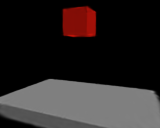
\includegraphics[width=.34\linewidth]{../../../output/npc-vision/4d4c8917622509ff51e06db391ab30b0c5af04dd86da6f865a96bfdb9482c96a/val-00.png}\hspace{5mm}
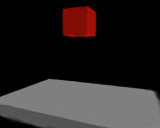
\includegraphics[width=.34\linewidth]{../../../output/npc-vision/4d4c8917622509ff51e06db391ab30b0c5af04dd86da6f865a96bfdb9482c96a/val-01.png}
\end{center}
这两张是重建结果。两个机位都没有参与训练，图中的箱子仍悬在烘焙时的位置。对两个机位分别与留出的原图比较，每个 RGB 分量先除以 255，再计算平方误差的平均值 $E$。按 $-10\log_{10} E$ 换算，分别为 31.64 和 31.86 dB。这个数衡量像素颜色的接近程度。箱子后来有没有落地，则需要在游戏运行时查证。

游戏调用 \code{AskNpcVision} 时给出场景名称和问题。视觉服务先根据机位的关键词选取至多两张图，再把图片、物体名称及编号交给视觉模型。示例中的名称与编号由关卡作者标注。服务只接受这几张图里列出的编号。候选列表用于缩小搜索范围，照片中不在列表里的物体需要先在资料中补上。

模型作答耗时可能跨越好几个物理步。游戏可以继续更新，等异步结果准备好，再在场景线程调用 \code{CanPickUp}。引擎按编号查找物体，检查“可拿取”组件，并从手的位置向物体发出一条长度有限的射线。如果中间已多了一面墙，射线会先碰到墙。如果箱子已被别人拿走，查实体时就会失败。这里返回的是此次查询的结果，游戏随后决定怎样改变物品栏或场景。

\clearpage
\subsection{照片中的区域与指向}

“指出地台右侧的灰色台面”问的是地台的一部分。场景里只有整座地台的编号，给右侧台面另建一个实体也无助于画面定位。关卡作者可以直接在照片上标出这块区域。下图的框保存在实验台的 \code{Physics-Workshop.views.json}，名称是“地台右侧的灰色台面”。

\begin{figure}[H]\centering
\begin{tikzpicture}[x=.37mm,y=-.37mm]
  \node[anchor=north west,inner sep=0] at (0,0)
    {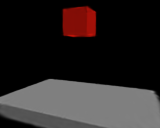
\includegraphics[width=59.2mm]{../../../output/npc-vision/4d4c8917622509ff51e06db391ab30b0c5af04dd86da6f865a96bfdb9482c96a/val-00.png}};
  \draw[yellow!85!white,line width=1.1pt] (108,96) rectangle (136,112);
  \fill[yellow!85!white] (122,104) circle[radius=1.2];
  \draw[blue,thick] (137,104) -- (173,104);
  \node[anchor=west,align=left,font=\small] at (175,104) {标注框中心 $(122,104)$\\左上角为 $(0,0)$};
\end{tikzpicture}
\caption{Brush 从重建的三维高斯渲染出机位 val-00，原图为 $160\times128$ 像素。黄色框与中心点按项目索引叠加。}
\end{figure}

照片中的一点只能确定一个观察方向。相机在世界坐标的 $(2.383,2.121,5.507)$，焦距折合 145 像素，光轴穿过图心 $(80,64)$。标注中心比图心向右 42 像素、向下 40 像素。在相机坐标里，向右为正 $x$，向上为正 $y$，镜头朝负 $z$。因此，从镜头出发，在正前方一个单位远的平面上，这个像素对应的位置是
\[
    \bigl((122-80)/145,\ (64-104)/145,\ -1\bigr).
\]
\code{bake\_npc\_views.py} 的 \code{region\_directions} 用拍摄时的相机旋转把这个向量转到世界坐标，再除以长度，得到 $(-0.106,-0.372,-0.922)$。在编辑器“NPC 观察”里按“从拍摄机位看向该处”，相机便回到照片的起点，沿这个方向观察。游戏中也可以把方向交给朝向或指示动作。换一个站位时须保留射线原来的起点，沿同一方向平移并不能保证指到原处。

测试利用场景中台面高度 $y=0$ 验算方向。照片射线与平面的交点约为 $(1.779,0,0.255)$，落在半宽 3 米、半深 2 米的台面内。交点只用于这间实验室的验证。普通单张照片没有给出目标距离，游戏取得的是从拍摄机位出发的世界射线。离线索引假定照片已经校正镜头畸变，机位和游戏采用同一套世界坐标。相机局部坐标与矩阵列的约定可对照 \href{https://docs.nerf.studio/quickstart/data_conventions.html}{Nerfstudio 的 Camera/view space 与 Camera extrinsics}。

\clearpage
\subsection{候选结果的读取与核验}

支持区域的游戏入口是 \code{AskNpcCandidate}。问“右边那个红箱子”仍然是在找箱子。服务选好图片，再把图中的实体和命中关键词的区域列在同一张表里。实验台里的箱子编号为 103，台面上的框在这次提问中暂用 104。模型选框时，服务把框内的实际像素裁出来再问一次。机位、框名、起点和方向都从已发图片的索引里取。模型自行报出的坐标、其他机位的引用和不存在的编号都会被丢弃。

游戏保留返回的 \code{future}，在后续更新中检查答案。下面是对应 \src{Redflag/src/Redflag/Scene/NpcVision.h}{NpcVision.h} 与 \src{RedflagForge/src/NpcVisionPanel.cpp}{NpcVisionPanel::Draw} 的调用节选；变量 \code{scene} 和 \code{camera} 是当前场景与编辑器相机。

\begin{lstlisting}[language=C++]
// (*@收到提问时保存 waiting，每次更新检查一次。@*)
if (waiting.valid() &&
    waiting.wait_for(std::chrono::seconds(0)) ==
    std::future_status::ready) {
    NpcVisionCandidate answer = waiting.get();
    if (answer.Region) {
        const NpcViewRegion& r = *answer.Region;
        camera.LookAt(r.Origin, r.Origin + r.Direction);
    } else if (answer.Entity) {
        bool reachable = CanPickUp(scene, *answer.Entity,
                                   hand, reachInMeters);
    }
}
\end{lstlisting}

调用 \code{get()} 会取走结果，后续更新通过 \code{valid()} 知道这次提问已经结束。正式面板还会检查提问时的场景是否仍然打开。只有持有实体编号并已启动物理模拟时，面板才调用拾取查询。两个字段都为空表示没有选出候选。C++ 游戏可以使用上述接口；目前分发的 C\# ScriptCore 只提供现有的实体变换和输入等脚本入口。

本机用 Qwen3-VL-2B 分别读了随仓图片和一次从头训练 800 步后导出的图片。在每组中用中文、英文各问一次，找台面时均选中右侧的框，找“右边的红箱子”时均选中实体 103。把两张图片第 65 行至底部涂黑，保留箱子和文字标签，模型在两种语言中均返回空。早期只让它选编号时，中文提问曾让模型在台面被遮掉后仍选中该处。裁图复查减少了这组样本里的误选。这里总共只有一处有标注的台面，同色材质、严重遮挡和换房间都需要另测。

\readings{\href{run:../npc-vision/regions.json}{逐项识图记录与图片校验值}\quad \href{https://repo-sam.inria.fr/fungraph/3d-gaussian-splatting/}{Kerbl 等，3D Gaussian Splatting，SIGGRAPH 2023}\quad
\href{https://github.com/ArthurBrussee/brush/releases/tag/v0.3.0}{Brush 0.3.0}\quad
\href{https://nvidia-omniverse.github.io/PhysX/physx/5.6.1/docs/SceneQueries.html}{PhysX 场景查询}}

\end{document}
